\documentclass[11pt,a4paper]{article}
\usepackage{amsthm,amsmath,amsfonts,exscale,latexsym,graphicx}
\usepackage{times}
%\usepackage[mtpcal,mtphrb,subscriptcorrection]{mtpro2}
\usepackage{natbib}
\usepackage[usenames]{color}
\usepackage[pagebackref,colorlinks=true,breaklinks,linkcolor=Gray,citecolor=Gray,urlcolor=Gray,bookmarks,pdfpagemode=UseOutlines,pdftitle={Project Proposal: Round Trip Loss for Machine Translation}]{hyperref}

\bibliographystyle{apalike}
%shortcuts
\def\beq{\begin{equation}}
\def\eeq{\end{equation}}
\begin{document}
\title{Round Trip Loss for Machine Translation}
\date{\today}
\author{
Anja Adamov$\mbox{}^a$\thanks{\emph{E-mail address:} adamova@student.ethz.ch},
Lauro B\"{o}ni$\mbox{}^b$\thanks{\emph{E-mail address:} laboeni@gmail.com},
Simon A.\ Broda$\mbox{}^c\mbox{}^d$\thanks{\emph{E-mail address:} simon.broda@uzh.ch},
Urs V\"{o}geli$\mbox{}^b$\thanks{\emph{E-mail address:} voegeli.urs@gmail.com}
\medskip \\
\textit{\small $\mbox{}^a$IBM Switzerland Ltd., Zurich, Switzerland}
\medskip \\
\textit{\small $\mbox{}^b$ETH Zurich}
\medskip \\
\textit{\small $\mbox{}^c$Department of Banking and Finance, University of Zurich}
\medskip \\
\textit{\small $\mbox{}^d$Quantitative Economics Section, University of Amsterdam}
}
\maketitle \setcounter{page}{0}\thispagestyle{empty}
\definecolor{Gray}{rgb}{0.5,0.5,0.5}
\begin{abstract}
We propose to augment a machine translation system by adding a round-trip loss which encourages the system to generate translations that when translated back into the source language, retain much of the original structure. We show that in doing so, the model will learn internal representations with improved semantic meaning.
\end{abstract}
\bigskip \textbf{Key Words}: Cycle consistency loss; deep learning; natural language understanding; machine translation; round-trip loss.
%\renewcommand{\baselinestretch}{1.3}\small\normalsize
\newpage
\setcounter{page}{1}
\section{Introduction}
Machine translation is an important task within the field of natural language understanding. Consequently, a variety of models have been proposed for solving it. One of the first truly successful models was the sequence-to-sequence (seq2seq) model of \citet{seq2seq}, while the current state of the art builds upon the \emph{Transformer} architecture introduced by \citet{transformer}. At a high level, both the seq2seq and the Transformer architectures are comprised of an encoder and decoder; the encoder learns an internal representation of the source sentence, and the decoder decodes it into the target language. For these models to work, the internal representation must capture the semantic meaning of the source sentence.

Irrespective of the architecture, these models are typically trained with the cross-entropy loss between the ground truth and predicted sentences, usually with teacher forcing.
Here, we propose to add a round-trip penalty to the loss function of the model. The idea is that instead of training a single model to translate from a source language $\mathcal{S}$ to a target language $\mathcal{T}$, one trains two models (of identical structure), one mapping $\mathcal{S}\mapsto \mathcal{T}$ and one mapping $\mathcal{T}\mapsto \mathcal{S}$. The two models are, at first, trained independently and in parallel, by feeding in the same batches of sentence pairs (in this paper, we rely on the Transformer architecture of \citet{transformer}, but the idea applies to any encoder-decoder architecture). After $\tau$ epochs, the models are then trained jointly, using as loss a sum of four cross-entropy terms, viz.,
\begin{equation}
\mathcal{L} = CE(s, \hat{s}) + CE(t, \hat{t}) + \lambda \left( CE(s, \tilde{s}) + CE(t, \tilde{t})\right).
\label{eq:RTL}
\end{equation}
Here, $s\in\mathcal{S}$ is the ground truth sentence in the first language, $t\in\mathcal{T}$ is the corresponding ground truth in the second language, $\hat{s}\in\mathcal{S}$ and $\hat{t}\in\mathcal{T}$ are the respective translations of $t$ and $s$, $\tilde{s}$ is obtained by translating $\hat{t}$ back to $\mathcal{S}$, and $\tilde{t}$ is obtained by translating $\hat{s}$ back to $\mathcal{T}$. $\tau$ and $\lambda$ are hyperparameters. 

The round-trip loss is inspired by the cycle consistency loss pioneered by \citet{CycleGAN2017} in the context of GANs. The only application of this concept to the field of machine translation of which we are aware is \citet{su:2018}, who adapt it for unsupervised multi-modal machine translation. Here, we propose to apply the idea to supervised machine translation. We conjecture that encouraging the model to generate round-trippable translations will help it learn a semantically meaningful representation. A related idea is that of back-translation, pioneered by \citet{backtrans}. \citeauthor{backtrans} propose to augment the parallel training corpus used to train a machine translation system with synthetic data, obtained by translating a monolingual corpus in the target language to the source language using an independently trained system. They argue that this is beneficial in particular when parallel training data is scarce. The difference with our approach is two-fold: i) in our approach, the two networks are trained \emph{jointly}, each with their own round-trip loss term, whereas in back-translation, the models are trained separately, with only one of them benefiting from back-translation; ii) we do not assume the existence of a separate monolingual corpus in the target language, but work strictly with a parallel corpus. Having ground truth available, we are thus able to use teacher forcing in constructing the round-trip loss contribution, greatly speeding up training.

The remainder of this manuscript is organized as follows. Section \ref{sec:models} describes the model architecture and our implementation of it. Section \ref{sec:results} details the results of our experiments with the proposed round-trip loss. Section \ref{sec:discussion} provides a discussion, and Section \ref{sec:conclusions} concludes.
\section{Models and Methods}\label{sec:models}
\subsection{Model Architecture}

This section is, unless explicitly stated otherwise, based on \cite{transformer}. Useful background information on Recurrent and Convolutional Neural Networks is based on \cite{Goodfellow-et-al-2016}.

The core idea behind the classical Transformer model is the so-called self-attention — the model's ability to attend to different positions of the input sequence to compute a representation of that sequence - without imposing any recurrence nor convolution to the model.

For deep neural networks aiming to perform sequence translation, some general sort of memory is required as, in practice, a lot of sequences depend on words from previous sequences. As an example for the reader, try to complete the phrases "My father is a winegrower. He likes to drink {\tt ...}". In this case, you might guess the missing word "wine" correctly - with the help of attention. And this is exactly, what modern natural language models try to capture.

Recurrent Neural Networks (short: RNN) tackle this problem by a specific architecture that focuses on time-dependencies. However, they are hardly or even not parallelizable and hence computationally suboptimal.
On the other hand, Convolution Neural Networks (short: CNN) are easily parallelizable and can exploit local dependencies. However, these models do not explicitly rely on the attention. 

\begin{figure}[ht]
    \centering
    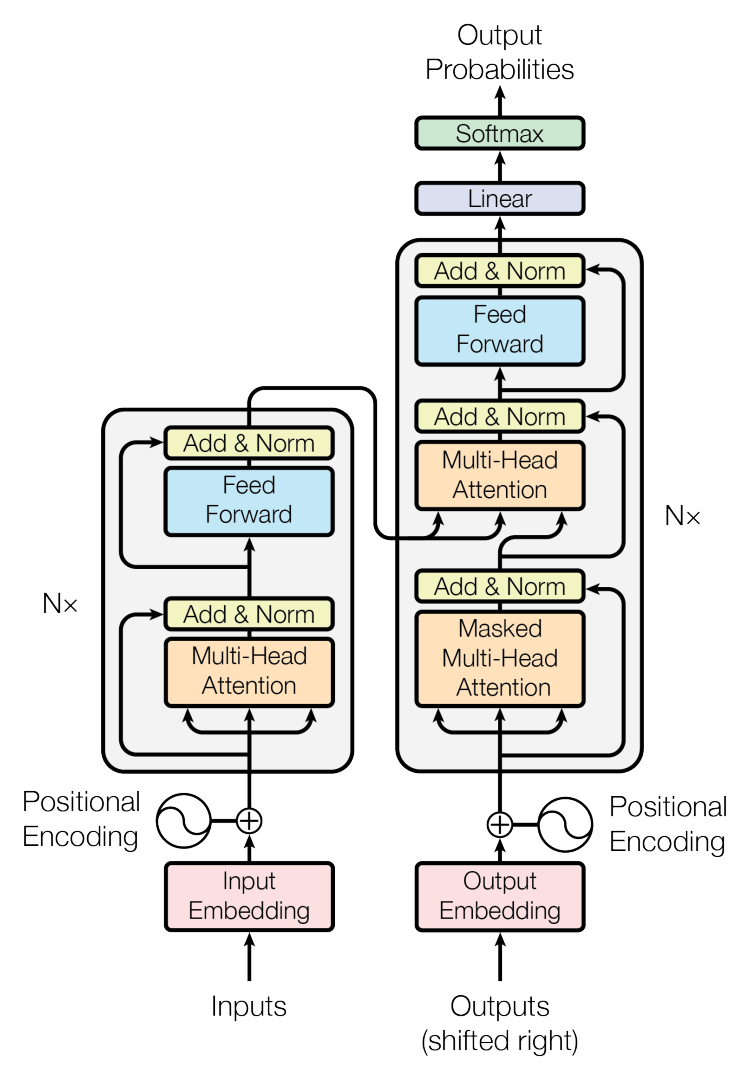
\includegraphics[scale=0.5]{images/Transformer.PNG}
    \caption{Architecture of the Transformer model from \cite{transformer}.}
    \label{fig:transformer}
\end{figure}

The Transformer model solely relies on attention - more precisely on self-attention - to capture global dependencies between input and output. In a nutshell, the model consists of a set of encoders (EC) and set of decoders (DC). The original model in (\citet{transformer}) uses $N=6$, i.e. 6-fold stacking of the respective ECs and DCs. Each EC maps input sequences $(x_1,...,x_n)$ to its continuous representation, say, $(z_1,...,z_n)$ which in turn are used by DCs to generate the output respective the translated prediction $(y_1,...,y_m)$.

More precisely, each EC consists of two components: self-attention and feed-forward neural networks (FNN). The self-attention mechanism takes in a set of input encodings of length $d_{\text{model}} = 512$ from the previous EC, splits it up to a key, value and query vector (each of length $d = 64$) and then tries to learn their relevance to each other to generate a set of output encodings, again of length $d_{\text{model}}$. The FNN then further processes each output encoding individually (the dimensionality of the input and output is therefore $d_{\text{model}}$, whereas the size of the inner-layer is $d_{\text{ff}} = 2048$). The output encodings are then finally passed to the next EC as its input, as well as to the DC.

On the other hand, each DC consists of three components: self-attention, an attention mechanism over the encodings and a classical FNN. The first EC takes positional information and embeddings of the input sequence as its input, rather than encodings. The positional information is necessary for the Transformer to make use of the order of the sequence, as it does not rely on recurrence nor convolution. Each DC functions in a similar fashion to the ECs, but an additional (masked) attention mechanism is inserted which draws relevant information from the encodings generated by the EC. Finally, the last DC is then followed by a linear transformation and a softmax layer to produce the desired output probabilities.

This somehow abstract description is visualized in Figure \ref{fig:transformer}. Moreover, Figure \ref{fig:attention} shows a visualization of the self-attention mechanism in the ECs where the relevance of each embedding (i.e. word) are compared.

\begin{figure}[ht]
    \centering
    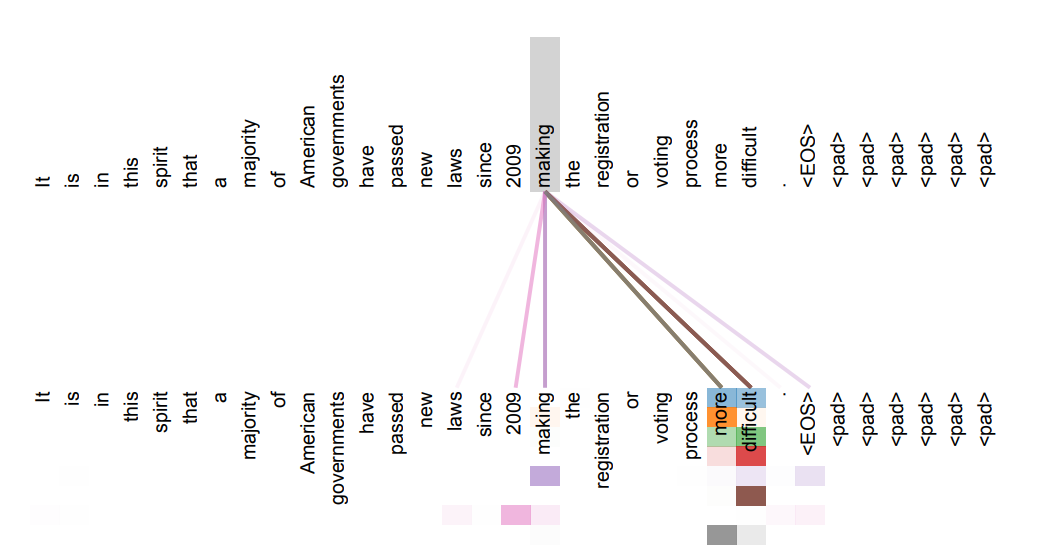
\includegraphics[scale=0.7]{images/attention.PNG}
    \caption{Visualization of the self-attention mechanism from \cite{transformer}.}
    \label{fig:attention}
\end{figure}

\subsection{Implementation and Training Details}
We use the Transformer implementation in TensorFlow 2.0 available from the \href{https://www.tensorflow.org/tutorials/text/transformer}{tensorflow website} and implement a custom training loop, which instantiates the $\mathcal{S}\mapsto\mathcal{T}$ and $\mathcal{T}\mapsto\mathcal{S}$ models and trains them jointly with the loss described in \eqref{eq:RTL}. We train our models on the WMT'14 English-German data set available from \href{https://nlp.stanford.edu/projects/nmt/}{https://nlp.stanford.edu/projects/nmt/}. The training set consists of 4,508,785 sentence pairs, of which we retain those where source and target sequence both have a length of 40 or fewer tokens to keep the computational demands manageable (the original Transformer model in \citet{transformer} uses a maximal sequence length of 65). We employ a subword tokenizer, and experiment with relatively small target vocabulary sizes of both $2^{13}$ and $2^{14}$, again to keep computational demands at bay (a production system would likely use a vocabulary at least twice as large). Compared to the base transformer, we also reduce the number of layers from from 6 to 4, $d_{model}$ from 512 to 128, and $d_{ff}$ from 2048 to 512. The number of attention heads is kept at 8.
With these choices, training the model (which consists of two transformers) for a single epoch on the entire dataset takes about ... on a single NVIDIA GTX1080 (?). We use a learning rate schedule that increases the learning rate from ... to ... over ... warm-up periods, and then decreases it again, down to a final value of ... 

At test time, we rely on the beam search decoder implementation from \href{https://github.com/tensorflow/tensor2tensor/blob/master/tensor2tensor/utils}{tensor2tensor}. We use a beam width of 10 and a length penalty of $\alpha=0.65$, per the recommendations of \citet{googlenmt}. The BLEU score for the 3,003 sentences in the test set is computed using the \href{https://www.nltk.org/}{nltk} package. 



%Based on the transformer implementation at \href{https://www.tensorflow.org/tutorials/text/transformer}{https://www.tensorflow.org/tutorials/text/transformer} we imposed a round-trip loss on the model based on the following definition: Let $\mathcal{S}$ be the original language (e.g. English) and $\mathcal{T}$ be the target language (e.g. German). The round-trip loss $\mathcal{L}_{\mathcal{S}, \mathcal{T}}$ from $\mathcal{S}$ to $\mathcal{T}$ and back to $\mathcal{S}$ is defined as
%\begin{equation}
%    \mathcal{L}_{\mathcal{S}, \mathcal{T}} (s,t) = \text{CE}(s, \hat{s}) + \text{CE}(t, \hat{t}) + \lambda %\left(\text{CE}(s, \tilde{s}) + \text{CE}(t, \tilde{t})\right),
%\end{equation}
%where $s \in \mathcal{S}$ is the ground truth sentences, $t \in \mathcal{T}$ is the corresponding ground truth in the second language, $\hat{s} = \text{Transformer}(t) \in \mathcal{S}$ and $\hat{t} = \text{Transformer}(s) \in \mathcal{T}$ are the respective predictions / translations of $t \in \mathcal{T}$ and $s \in \mathcal{S}$. $\tilde{s}$ and $\tilde{t}$ are obtained by translating $\hat{t}$ and $\hat{s}$ back to $\mathcal{S}$ and $\mathcal{T}$. $\text{CE}$ stands for the cross-entropy and $\lambda$ is a hyperparameter. 

%More formally, we have
%\begin{equation}
%    s \in \mathcal{S} \longmapsto{} \hat{t} \in \mathcal{T} \longmapsto{} \tilde{s} \in \mathcal{S}
%\end{equation}
%\begin{equation}
%    t \in \mathcal{T} \longmapsto{} \hat{s} \in \mathcal{S} \longmapsto{} \tilde{t} \in \mathcal{T}.
%end{equation}
%Hence $\mathcal{L}_{\mathcal{S}, \mathcal{T}}$ represents the sum of the respective cross-entropies between the ground truth and its predictions and the ground truth and the twice-translated sentences. Note that $\mathcal{L}_{\mathcal{S}, \mathcal{T}}$ is bidirectional.

\textbf{TODO: implementation of backtranslation}

\section{Results}\label{sec:results}
\subsection{Experiments}
In order to evaluate the effect of our proposed round-trip loss, we conduct a number of experiments. First, we train and evaluate the model from scratch for different values of $\lambda$. This corresponds to setting $\tau=0$ in \eqref{eq:RTL}. The results after training each model for 15 epochs are shown in Table ...

Next, we pre-train a model with $\lambda=0$ for 15 epochs, and then fine-tune it for another 15 epochs using the same values for $\lambda$ as before. The results are shown in Table ...

Finally, in order to compare our approach to the back-translation approach of \citet{backtrans}, ...
\subsection{Example Translations}
\section{Discussion}\label{sec:discussion}
Discuss the strengths and weaknesses of your approach, based on the results. Point out the implications of your novel idea on the application concerned.
\section{Summary}\label{sec:conclusions}
Summarize your contributions in light of the new results.
\bibliography{proposal}
\end{document}

